\section{Considerações Finais}

Enviamos o código para o ESP32 utilizando o comando \textit{Alt + Ctrl + U}. Em certos casos, é preciso apertar o botão de BOOT para enviar. Feito o envio, as cores devem aparecer no LED RGB.

\begin{figure}
    \centering
    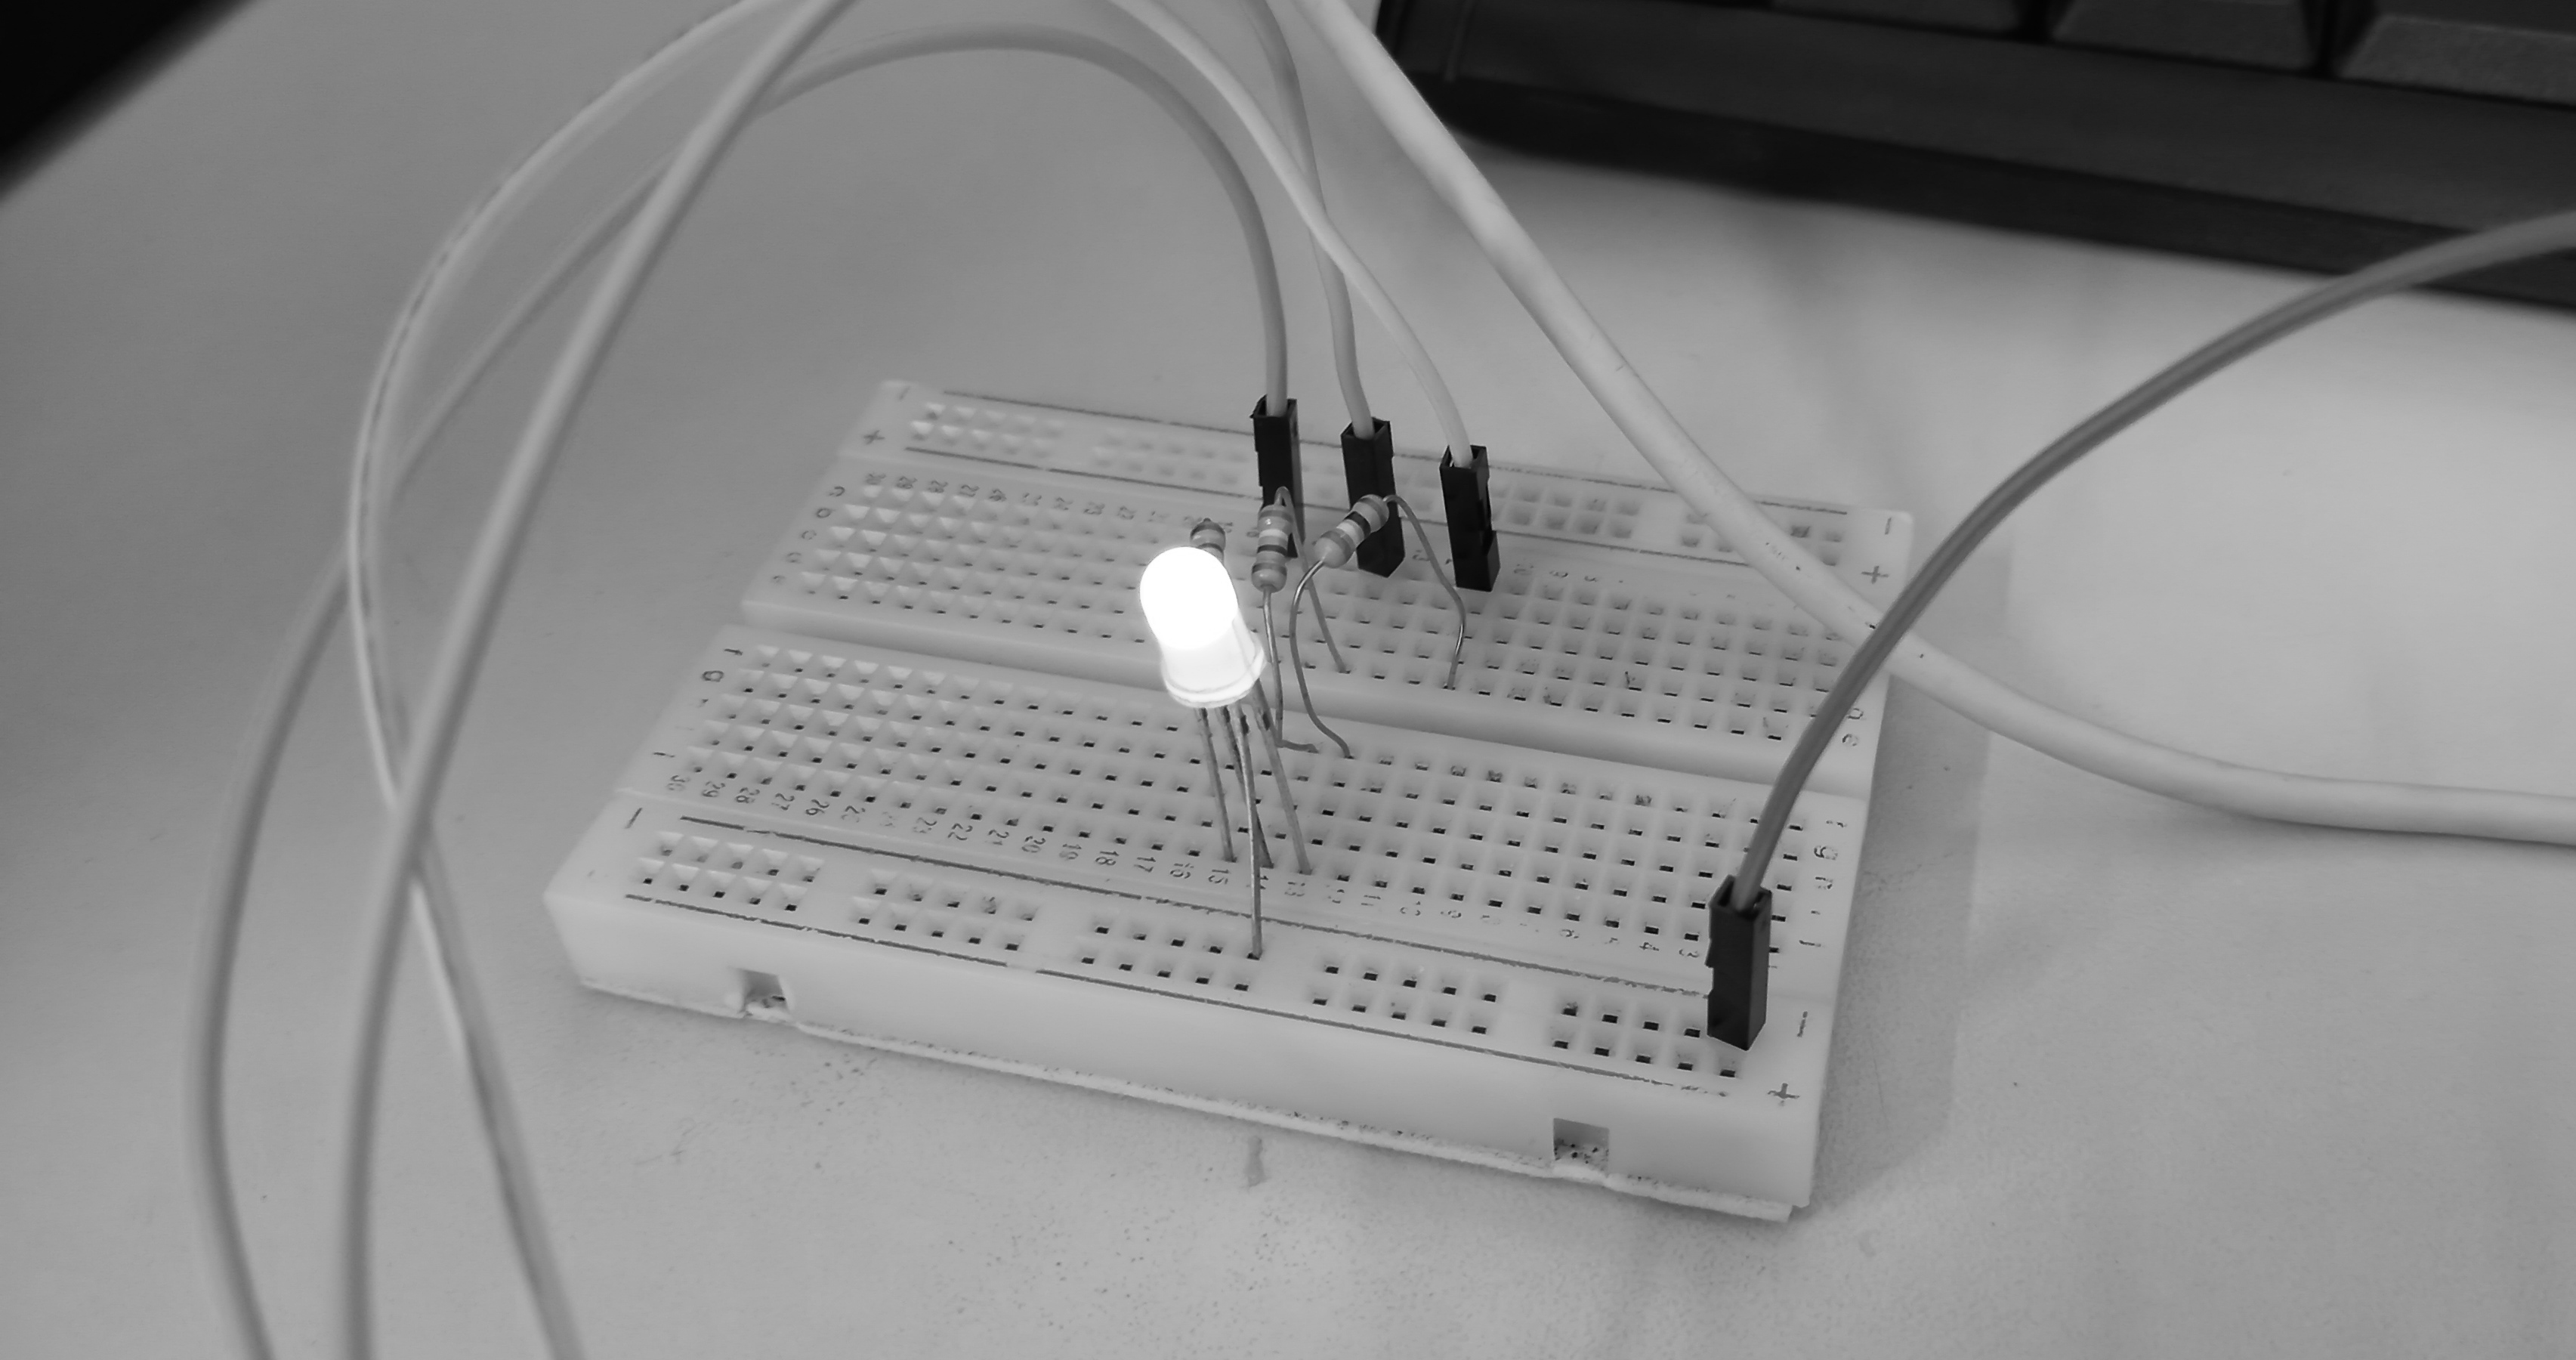
\includegraphics[width=0.5\linewidth]{img/final_result.jpg}
    \caption{Resultado final.}
    \label{fig:final-result}
\end{figure}

Para conferir o código completo, acesse esse \href{https://github.com/fabricio-araujo94/microcontroladores/tree/main/pwm_}{link} para o repositório no GitHub. Para ver o resultado da prática em execução, assista esse \href{https://youtu.be/cyvFmMO40j8}{vídeo} no YouTube.